\documentclass[landscape,twocolumn,letterpaper,9pt,reqno]{article}\usepackage[]{graphicx}\usepackage[]{color}
%% maxwidth is the original width if it is less than linewidth
%% otherwise use linewidth (to make sure the graphics do not exceed the margin)
\makeatletter
\def\maxwidth{ %
  \ifdim\Gin@nat@width>\linewidth
    \linewidth
  \else
    \Gin@nat@width
  \fi
}
\makeatother

\definecolor{fgcolor}{rgb}{0.345, 0.345, 0.345}
\newcommand{\hlnum}[1]{\textcolor[rgb]{0.686,0.059,0.569}{#1}}%
\newcommand{\hlstr}[1]{\textcolor[rgb]{0.192,0.494,0.8}{#1}}%
\newcommand{\hlcom}[1]{\textcolor[rgb]{0.678,0.584,0.686}{\textit{#1}}}%
\newcommand{\hlopt}[1]{\textcolor[rgb]{0,0,0}{#1}}%
\newcommand{\hlstd}[1]{\textcolor[rgb]{0.345,0.345,0.345}{#1}}%
\newcommand{\hlkwa}[1]{\textcolor[rgb]{0.161,0.373,0.58}{\textbf{#1}}}%
\newcommand{\hlkwb}[1]{\textcolor[rgb]{0.69,0.353,0.396}{#1}}%
\newcommand{\hlkwc}[1]{\textcolor[rgb]{0.333,0.667,0.333}{#1}}%
\newcommand{\hlkwd}[1]{\textcolor[rgb]{0.737,0.353,0.396}{\textbf{#1}}}%
\let\hlipl\hlkwb

\usepackage{framed}
\makeatletter
\newenvironment{kframe}{%
 \def\at@end@of@kframe{}%
 \ifinner\ifhmode%
  \def\at@end@of@kframe{\end{minipage}}%
  \begin{minipage}{\columnwidth}%
 \fi\fi%
 \def\FrameCommand##1{\hskip\@totalleftmargin \hskip-\fboxsep
 \colorbox{shadecolor}{##1}\hskip-\fboxsep
     % There is no \\@totalrightmargin, so:
     \hskip-\linewidth \hskip-\@totalleftmargin \hskip\columnwidth}%
 \MakeFramed {\advance\hsize-\width
   \@totalleftmargin\z@ \linewidth\hsize
   \@setminipage}}%
 {\par\unskip\endMakeFramed%
 \at@end@of@kframe}
\makeatother

\definecolor{shadecolor}{rgb}{.97, .97, .97}
\definecolor{messagecolor}{rgb}{0, 0, 0}
\definecolor{warningcolor}{rgb}{1, 0, 1}
\definecolor{errorcolor}{rgb}{1, 0, 0}
\newenvironment{knitrout}{}{} % an empty environment to be redefined in TeX

\usepackage{alltt}

\usepackage{lscape,fancyhdr}

\usepackage{hyperref}
\usepackage{float}
\pagestyle{fancy}

\usepackage{amsmath,epsfig,subfigure,amsthm,amsfonts,epsf,psfrag,rotating,setspace,bm}

\usepackage{verbatim,color} % Allow text colors}
\usepackage{placeins}

\setlength{\oddsidemargin}{-0.4in}		% default=0in
\setlength\evensidemargin{-0.4in}

\setlength{\textwidth}{9.8in}		% default=9in

\setlength{\columnsep}{0.5in}		% default=10pt

\setlength{\columnseprule}{0pt}		% default=0pt (no line)


\setlength{\textheight}{7.0in}		% default=5.15in

\setlength{\topmargin}{-0.75in}		% default=0.20in

\setlength{\headsep}{0.25in}		% default=0.35in

\setlength{\parskip}{1.2ex}

\setlength{\parindent}{0mm}

\newcommand{\compresslist}{ % Define a command to reduce spacing within itemize/enumerate environments, this is used right after \begin{itemize} or \begin{enumerate}
	\setlength{\itemsep}{1pt}
	\setlength{\parskip}{0pt}
	\setlength{\parsep}{0pt}
}


\lhead{Course EPIB607: Regression handout 006 (Logistic regression - HIV and Smoking examples)}
\rhead{jh,sb \ \ \ v. 2018.11.26}
\IfFileExists{upquote.sty}{\usepackage{upquote}}{}
\begin{document}
	



\section{Mean depth of the ocean}




The \texttt{depths} dataset shown below contains the depths of the ocean in the \texttt{alt} column and whether the sampled location is in the northern or southern hemisphere given by the \texttt{South} column (South=0 is the north and South=1 is the south). There are 200 samples from the north and 200 from the south. 

\begin{knitrout}
\definecolor{shadecolor}{rgb}{0.969, 0.969, 0.969}\color{fgcolor}
\begin{alltt}
\hlkwd{head}\hlstd{(depths)}
\end{alltt}
\begin{verbatim}
##           X        lon       lat  alt water South
## 41995 41995  -87.21236 59.290367  190     1     0
## 11151 11151 -122.33034  5.554558 4167     1     0
## 43640 43640 -148.54790 36.237464 5447     1     0
## 8615   8615  -24.92364 21.625967 5063     1     0
## 8126   8126  177.18458 13.880370 5634     1     0
## 16548 16548   48.88215  3.229250 3691     1     0
\end{verbatim}
\begin{alltt}
\hlkwd{dim}\hlstd{(depths)}
\end{alltt}
\begin{verbatim}
## [1] 400   6
\end{verbatim}

\end{knitrout}

\begin{knitrout}
\definecolor{shadecolor}{rgb}{0.969, 0.969, 0.969}\color{fgcolor}
\begin{verbatim}
## Coefficients:
##             Estimate Std. Error t value Pr(>|t|)    
## (Intercept)  3683.52      78.71    46.8   <2e-16 ***
## ---
## Signif. codes:  0 '***' 0.001 '**' 0.01 '*' 0.05 '.' 0.1 ' ' 1
## 
## Residual standard error: 1574 on 399 degrees of freedom
\end{verbatim}

\end{knitrout}

\begin{enumerate}\compresslist
	\item A linear regression output is shown. What type of regression is this?
	\item What is the sample size? 
	\item What is the parameter of interest?
	\item How many determinants are there for the parameter of interest?
	\item Give the regression equation in terms of population parameters. Define each of the parameters in your model.
		\item Provide the \texttt{R} code used to fit the regression equation.
	\item What does the \texttt{Estimate} for \texttt{(Intercept)} represent? Would it be possible to calculate this value without running a regression? If yes, how?
	\item How is the \texttt{Std. Error} calculated?
	\item Show how the \texttt{t value} was calculated. State the implied hypothesis test. 
	\item Show how the \texttt{p-value} was calculated.
	\item Calculate a 95\% confidence interval for the parameter of interest. State the assumptions you used to calculate this CI.
\end{enumerate}



\clearpage

\section{Mean depth of the ocean in northern and southern hemisphere}

\begin{knitrout}
\definecolor{shadecolor}{rgb}{0.969, 0.969, 0.969}\color{fgcolor}

{\centering 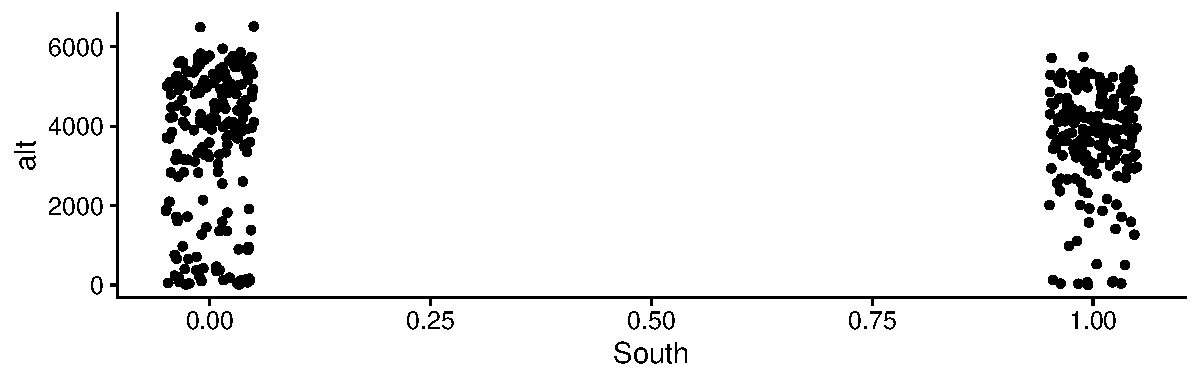
\includegraphics[width=1\linewidth]{figure/unnamed-chunk-4-1} 

}



\end{knitrout}


\begin{knitrout}\footnotesize
\definecolor{shadecolor}{rgb}{0.969, 0.969, 0.969}\color{fgcolor}
\begin{verbatim}
## Coefficients:
##             Estimate Std. Error t value Pr(>|t|)    
## (Intercept)  3643.08     111.42  32.698   <2e-16 ***
## South          80.88     157.56   0.513    0.608    
## ---
## Signif. codes:  0 '***' 0.001 '**' 0.01 '*' 0.05 '.' 0.1 ' ' 1
## 
## Residual standard error: 1576 on 398 degrees of freedom
## Multiple R-squared: 0.0006617,	Adjusted R-squared: -0.001849 
## F-statistic: 0.2635 on 1 and 398 DF,  p-value: 0.608
\end{verbatim}
\begin{alltt}
\hlkwd{t.test}\hlstd{(alt} \hlopt{~} \hlstd{South,} \hlkwc{data} \hlstd{= depths,} \hlkwc{var.equal} \hlstd{=} \hlnum{TRUE}\hlstd{)}
\end{alltt}
\begin{verbatim}
##  Two Sample t-test with alt by South 
## t = -0.5133, df = 398, p-value = 0.608
## alternative hypothesis: true difference in means is not equal to 0 
## 95 percent confidence interval:
##  -390.6487  228.8787 
## sample estimates:
## mean in group 0 mean in group 1 
##        3643.080        3723.965
\end{verbatim}

\end{knitrout}


\begin{enumerate}\compresslist
	\item A linear regression output is shown. What is the parameter of interest?
	\item How many determinants are there for the parameter of interest?
	\item Give the regression equation in terms of population parameters. Define each of the parameters in your model.
	\item Provide the \texttt{R} code used to fit the regression equation.
	\item What does the \texttt{Estimate} for \texttt{South} represent? Would it be possible to calculate this value without running a regression? If yes, how?
	\item Show how the \texttt{t value} for \texttt{South} was calculated. State the implied hypothesis test. 
	\item Show how the \texttt{p-value} was calculated. Interpret this p-value in the context of the problem. 
	\item Calculate a 95\% confidence interval for the parameter of interest. State the assumptions you used to calculate this CI.
\end{enumerate}


\clearpage

\section{Ratio depth of the ocean in northern and southern hemisphere}

\begin{knitrout}
\definecolor{shadecolor}{rgb}{0.969, 0.969, 0.969}\color{fgcolor}
\begin{verbatim}
## 
## Coefficients:
##             Estimate Std. Error t value Pr(>|t|)    
## (Intercept)  8.20058    0.03058 268.144   <2e-16 ***
## South        0.02196    0.04278   0.513    0.608    
## ---
## Signif. codes:  0 '***' 0.001 '**' 0.01 '*' 0.05 '.' 0.1 ' ' 1
## 
## (Dispersion parameter for gaussian family taken to be 2482673)
## 
##     Null deviance: 988758010  on 399  degrees of freedom
## Residual deviance: 988103771  on 398  degrees of freedom
## AIC: 7029.1
## 
## Number of Fisher Scoring iterations: 5
\end{verbatim}

\end{knitrout}


\begin{enumerate}\compresslist
	\item A linear regression output is shown. What is the parameter of interest?
	\item Give the regression equation in terms of population parameters. Define each of the parameters in your model.
	\item Provide the \texttt{R} code used to fit the regression equation.
	\item What does the \texttt{Estimate} for \texttt{South} represent? Would it be possible to calculate this value without running a regression? If yes, how?
	\item State the implied hypothesis test. Show how the \texttt{p-value} was calculated. Interpret this p-value in the context of the problem. 
	\item Calculate a 95\% confidence interval for the \% difference between the depths of the ocean in the South vs the North. 
	\item Are the depths of the ocean different in the South compared to the North? Explain. 
\end{enumerate}


\clearpage


\section{Student drinking}

A professor asked her sophomore students, “How many drinks do you typically have per session” (A drink is defined as one 12-ounce
beer, one 4-ounce glass of wine, or one 1-ounce shot of liquor.) Some of the students didn’t drink. Below are two fitted regressions based on the responses of the female and male students who did drink. \texttt{gender=1} is male and \texttt{gender=0} is female. 



\begin{knitrout}\footnotesize
\definecolor{shadecolor}{rgb}{0.969, 0.969, 0.969}\color{fgcolor}
\begin{alltt}
\hlstd{fit} \hlkwb{<-} \hlkwd{lm}\hlstd{(drinks} \hlopt{~} \hlstd{gender,} \hlkwc{data} \hlstd{= drinks)}
\hlkwd{summary}\hlstd{(fit)}
\end{alltt}
\begin{verbatim}
## Coefficients:
##             Estimate Std. Error t value Pr(>|t|)    
## (Intercept)   4.2947     0.2837  15.138  < 2e-16 ***
## gender        2.2238     0.4182   5.318  3.2e-07 ***
## ---
## Signif. codes:  0 '***' 0.001 '**' 0.01 '*' 0.05 '.' 0.1 ' ' 1
## 
## Residual standard error: 2.765 on 174 degrees of freedom
## Multiple R-squared: 0.1398,	Adjusted R-squared: 0.1348 
## F-statistic: 28.28 on 1 and 174 DF,  p-value: 3.197e-07
\end{verbatim}
\begin{alltt}
\hlstd{fit} \hlkwb{<-} \hlkwd{glm}\hlstd{(drinks} \hlopt{~} \hlstd{gender,} \hlkwc{data} \hlstd{= drinks,} \hlkwc{family} \hlstd{=} \hlkwd{gaussian}\hlstd{(}\hlkwc{link}\hlstd{=log))}
\hlkwd{summary}\hlstd{(fit)}
\end{alltt}
\begin{verbatim}
## 
## Coefficients:
##             Estimate Std. Error t value Pr(>|t|)    
## (Intercept)  1.45739    0.06606  22.062  < 2e-16 ***
## gender       0.41726    0.08115   5.142 7.27e-07 ***
## ---
## Signif. codes:  0 '***' 0.001 '**' 0.01 '*' 0.05 '.' 0.1 ' ' 1
## 
## (Dispersion parameter for gaussian family taken to be 7.646385)
## 
##     Null deviance: 1546.7  on 175  degrees of freedom
## Residual deviance: 1330.5  on 174  degrees of freedom
## AIC: 861.48
## 
## Number of Fisher Scoring iterations: 5
\end{verbatim}

\end{knitrout}


\begin{enumerate}\compresslist
	\item Two linear regression outputs are shown. For each, what is the parameter of interest?
	\item For each, give the regression equation in terms of population parameters. Define each of the parameters in your model.
	\item What does the \texttt{Estimate} for \texttt{gender} represent in each regression? Would it be possible to calculate this value without running a regression? If yes, how?
	\item State the implied hypothesis test. Show how the \texttt{p-value} was calculated. Interpret this p-value in the context of the problem. 
	\item Calculate a 95\% confidence interval for the \% difference between the number of drinks in males vs females. 
	\item Are the number of drinks different in males vs. females? Explain. 
\end{enumerate}


\clearpage

\section{Breastfeeding and respiratory infection I}

A total of 189,612 person-years of follow up were accumulated over the course of the study: 151,690
among infants who were being breastfed and 37,922 among infants not being breastfed. Over the
course of follow up the investigators identified 514,230 incident cases of respiratory infection among
breastfeeding infants and 140,312 among non-breastfeeding infants. Calculate the crude incidence rate difference and 95\% CI comparing infants who were not breastfed with those who were.

\begin{knitrout}\small
\definecolor{shadecolor}{rgb}{0.969, 0.969, 0.969}\color{fgcolor}
\begin{alltt}
\hlstd{fit} \hlkwb{<-} \hlkwd{glm}\hlstd{(cases} \hlopt{~ -}\hlnum{1} \hlopt{+} \hlstd{PT} \hlopt{+} \hlstd{PT}\hlopt{:}\hlstd{not_breastfed,} \hlkwc{family} \hlstd{=} \hlkwd{poisson}\hlstd{(}\hlkwc{link} \hlstd{= identity))}
\hlkwd{summary}\hlstd{(fit)}
\end{alltt}
\begin{verbatim}
## 
## Coefficients:
##                  Estimate Std. Error z value Pr(>|z|)    
## PT               3.390006   0.004727  717.10   <2e-16 ***
## PT:not_breastfed 0.310010   0.010951   28.31   <2e-16 ***
## ---
## Signif. codes:  0 '***' 0.001 '**' 0.01 '*' 0.05 '.' 0.1 ' ' 1
## 
## (Dispersion parameter for poisson family taken to be 1)
## 
##     Null deviance:        Inf  on 2  degrees of freedom
## Residual deviance: 1.1195e-10  on 0  degrees of freedom
## AIC: 32.678
## 
## Number of Fisher Scoring iterations: 2
\end{verbatim}

\end{knitrout}

\begin{enumerate}\compresslist
	\item Give the implied regression equation in terms of population parameters. Define each of the parameters in your model.
	\item What does the \texttt{Estimate} for \texttt{PT} and \texttt{PT:not\_breastfed} each represent? 
	\item Explain why there is a \texttt{-1} in the \texttt{glm} formula.
\end{enumerate}



\clearpage




\section{Breastfeeding and respiratory infection II}

A total of 189,612 person-years of follow up were accumulated over the course of the study: 151,690
among infants who were being breastfed and 37,922 among infants not being breastfed. Over the
course of follow up the investigators identified 514,230 incident cases of respiratory infection among
breastfeeding infants and 140,312 among non-breastfeeding infants. Calculate the crude incidence rate difference and 95\% CI comparing infants who were not breastfed with those who were. We are interested in calculating the incidence rate ratio and 95\% CI comparing infants who were not breastfed with those who were.




\begin{enumerate}\compresslist
	\item What is the parameter of interest?
	\item Give the regression equation in terms of the population parameters including the parameter of interest. Define each of the parameters in your model.
	\item How would you fit this model in \texttt{R}? First show what the data looks like, and then provide the \texttt{R} code to fit the regression model given in part 2.
	\item The fitted regression equation is given by: \[ \widehat{\log(\mu)} = 1.22 + 0.0875 \cdot NBF + \log(PT) \] where $\mu$ is the expected number of cases of respiratory infection, $NBF=1$ if not breastfed and 0 otherwise, and $PT$ is the person time in years. Calculate the fitted values, i.e., the expected number of cases, for both the not breastfed and breastfed group. Do you notice anything in particular about these fitted values? If yes, explain. 
\end{enumerate}


\clearpage


\section{Malaria control with bednets}

See the 2018 Lancet article \textit{Efficacy of Olyset Duo, a bednet containing pyriproxyfen and permethrin, versus a permethrin-only net against clinical malaria in an area with highly pyrethroid-resistant vectors in rural Burkina Faso: a cluster-randomised
	controlled trial} (\texttt{Bednets.pdf} in \texttt{A9} folder of myCourses) by Tiono et. al. exposure=1 is the new bednet, and exposure=0 is the existing bednet. A poisson regression with log link is fitted to the data and provides the following output:




\begin{knitrout}
\definecolor{shadecolor}{rgb}{0.969, 0.969, 0.969}\color{fgcolor}
\begin{verbatim}
## 
## Coefficients:
##             Estimate Std. Error z value Pr(>|z|)    
## (Intercept)  0.68314    0.02432  28.092  < 2e-16 ***
## exposure    -0.26687    0.03286  -8.121 4.62e-16 ***
## ---
## Signif. codes:  0 '***' 0.001 '**' 0.01 '*' 0.05 '.' 0.1 ' ' 1
## 
## (Dispersion parameter for poisson family taken to be 1)
## 
##     Null deviance: 1381.2  on 23  degrees of freedom
## Residual deviance: 1316.0  on 22  degrees of freedom
## AIC: 1476.7
## 
## Number of Fisher Scoring iterations: 5
\end{verbatim}

\end{knitrout}





\begin{enumerate}\compresslist
	\item What is the regression equation in terms of population parameters? Define all your parameters. 
	\item What is the fitted regression equation for the expected counts of malaria cases?
	\item What is the rate ratio and 95\% CI comparing PPF-treated (exposure=1) to Standard long-lasting insecticidal (exposure=0) nets?
	\item Do you expect this model to be a good fit for the data in Table 2? Explain why or why not.
\end{enumerate}


\clearpage


\section{Population mortality rates in Denmark}
\small 

\vspace*{-.1in}

We can fit the following simple (multiplicative) rate ratio model to the 
patterns of mortality rates  for 1980-1984 and  2000-2004. The reference cell is females 70-74,   1980-84. $R$ = rate. $M$ = multiplier.

\begin{tabular}{|l c | l l  l  l  | l l l l | l |}
	\hline
	Year  & Age & \multicolumn{3}{c}{Female (F)} & &   \multicolumn{3}{c}{Male (M)} & \\ 
	\hline
	& 70-74 &  $R_{F}$ & & & & $R_{F}$ & & $\times M_{M}$  & \\
	1980- & 75-79 &  $R_{F}$ & $ \times M_{75}$ & &   & $R_{F}$ & $\times M_{75}$ & $\times M_{M}$ & \\
	1984 & 80-84 & $R_{F}$ & $ \times M_{80}$ &  & &  $R_{F}$ & $ \times M_{80}$ & $ \times M_{M}$ & \\
	& 85-89 & $R_{F}$ & $ \times M_{85}$ &  & &  $R_{F}$ & $ \times M_{85}$ & $ \times M_{M}$ & \\ 
	\hline
	& 70-74 &  $R_{F}$ &  & & $\times M_{20y}$  &  $R_{F}$ & & $  \times M_{M}$  & $\times M_{20y}$\\
	2000- & 75-79 &  $R_{F} $ & $\times M_{75}$ & & $\times M_{20y}$ &  $R_{F}$ & $ \times M_{75}$ & $ \times M_{M}$& $\times M_{20y}$ \\
	2004      & 80-84 & $R_{F}$ & $ \times M_{80}$ & & $\times M_{20y}$ &   $R_{F}$ & $ \times M_{80}$ & $ \times M_{M}$ & $\times M_{20y}$ \\
	& 85-89 & $R_{F}$ & $ \times M_{85}$ & \ \ \ & $\times M_{20y}$&   $R_{F}$ & $\times M_{85}$ & $\times M_{M}$ & $\times M_{20y}$ \\
	\hline
\end{tabular}

%The array called `r' in the R code ( which fits additive models to the rates and logs of the rates)can be used to calculate ratios.

\begin{knitrout}
\definecolor{shadecolor}{rgb}{0.969, 0.969, 0.969}\color{fgcolor}
\begin{tabular}{l|l|r|r|r|r|r|r}
\hline
Year & Age & Female\_deaths & Female\_PT & Female\_rate & Male\_deaths & Male\_PT & Male\_rate\\
\hline
1980-1984 & 70-74 & 15989 & 586882.8 & 0.0272439 & 23810 & 456908.21 & 0.0521111\\
\hline
1980-1984 & 75-79 & 20838 & 454142.7 & 0.0458843 & 24707 & 300318.92 & 0.0822692\\
\hline
1980-1984 & 80-84 & 24073 & 297678.6 & 0.0808691 & 20319 & 167303.51 & 0.1214499\\
\hline
1980-1984 & 85-89 & 20216 & 147771.7 & 0.1368057 & 13524 & 74295.83 & 0.1820291\\
\hline
2000-2004 & 70-74 & 13912 & 521561.9 & 0.0266737 & 17360 & 436994.92 & 0.0397259\\
\hline
2000-2004 & 75-79 & 19731 & 471945.5 & 0.0418078 & 22477 & 341362.82 & 0.0658449\\
\hline
2000-2004 & 80-84 & 25541 & 369989.9 & 0.0690316 & 22992 & 217929.72 & 0.1055019\\
\hline
2000-2004 & 85-89 & 27135 & 226798.1 & 0.1196439 & 17444 & 104009.58 & 0.1677153\\
\hline
2005-2009 & 70-74 & 12179 & 540568.6 & 0.0225300 & 15782 & 472012.84 & 0.0334355\\
\hline
2005-2009 & 75-79 & 17273 & 444474.2 & 0.0388616 & 19547 & 344351.34 & 0.0567647\\
\hline
2005-2009 & 80-84 & 23513 & 363534.1 & 0.0646789 & 21781 & 230530.24 & 0.0944822\\
\hline
2005-2009 & 85-89 & 26842 & 237877.3 & 0.1128397 & 17811 & 114485.04 & 0.1555749\\
\hline
\end{tabular}


\end{knitrout}

%The equation is for the rate in any given age-group in a given gender in a given calendar period:
\textcolor{white}{text}\newline

\begin{tabular}{c c c c c c c c c}
	Rate = & $\rule{1cm}{0.15mm}$ & $\times \rule{1cm}{0.15mm}$ & $\times \rule{1cm}{0.15mm}$ & $\times \rule{1cm}{0.15mm}$ & $\times \rule{1cm}{0.15mm}$ & $\times \rule{1cm}{0.15mm}$ \\
	& &   if  &  if &  if & if & if & \\
	& &  75-79 & 80-84 & 85-89 & male & 2000-04 \\  \\
	$\log[Rate] =$ & $\rule{1cm}{0.15mm}$ & $+ \rule{1cm}{0.15mm}$ & $+ \rule{1cm}{0.15mm}$ & $+ \rule{1cm}{0.15mm}$ & $+ \rule{1cm}{0.15mm}$ & $+ \rule{1cm}{0.15mm}$ \\
	& &   if  &  if &  if & if & if & \\
	& &  75-79 & 80-84 & 85-89 & male & 2000-04 \\ \\
	
	$\log[Rate] =$ &$\rule{1cm}{0.15mm}$& $+  \rule{1cm}{0.15mm}$ & $+   \rule{1cm}{0.15mm}$ & $+   \rule{1cm}{0.15mm}$ & $+   \rule{1cm}{0.15mm} $ & $+ \rule{1cm}{0.15mm}$ \\
	& &  $\times$  &  $\times$ &  $\times$ & $\times$ & $\times$ & \\
	& &  $I_{75-79}$ & $I_{80-84}$ & $I_{85-89}$ & $I_{male}$ & $I_{2000-04}$ \\
\end{tabular}

where each $`I'$ is a (0/1) indicator of the category in question. By using both the 0 and 1 values of each $I$, this 6-parameter equation  produces a fitted value for each of the $4\times2\times2=16$ cells.

%You can also think of $I_{75-79},$  $I_{80-84},$ and  $I_{85-89}$ as 
%`radio buttons':  at most 1 of them can be `on' at the same time, since there are 4 
%age levels in all.


\begin{enumerate}\compresslist
	\item How many determinants are there for the mortality rate? How many parameters are required to represent these determinants?
	\item Estimate the parameters using a calculator, and fill in the blanks in the regression equations. 
	\item Interpret the estimate for the $M_{80}$ parameter.
	\item Fill in the blanks: The corresponding regression equation would reparametrize $\rule{1cm}{0.15mm}$ parameters as a function of $\rule{1cm}{0.15mm}$ parameters.
\end{enumerate}

\clearpage


\section{Kidney stone removal procedures 1}
The 1986 BMJ article \textit{Comparison of treatment of renal calculi by open surgery, percutaneous nephrolithotomy, and extracorporeal shockwave lithotripsy} by Charig et. al, was a study designed to compare different methods of treating kidney stones in order to establish which was the most cost effective and successful. The procedure, either open surgery, or percutaneous nephrolithotomy (PN, a keyhole surgery procedure), was defined to be successful if stones were eliminated or reduced to less than 2 mm after three months. The study collected cases of kidney stones treated at a particular UK hospital during 1972-1985. The counts of successes for the two surgical procedures were:

\begin{table}[h]
	\centering
	\begin{tabular}{lcc|c}
		& Unsuccessful &  Successful & Total\\
		Open surgery & 77 & 273 & 350 \\
		PN & 61 & 289 & 350 \\
		\hline
		Total & 138 & 562 & 700
	\end{tabular}
\end{table}


\begin{knitrout}
\definecolor{shadecolor}{rgb}{0.969, 0.969, 0.969}\color{fgcolor}
\begin{verbatim}
## 
## Coefficients:
##             Estimate Std. Error z value Pr(>|z|)    
## (Intercept)  -1.5556     0.1409 -11.040   <2e-16 ***
## open          0.2899     0.1911   1.517    0.129    
## ---
## Signif. codes:  0 '***' 0.001 '**' 0.01 '*' 0.05 '.' 0.1 ' ' 1
## 
## (Dispersion parameter for binomial family taken to be 1)
## 
##     Null deviance: 2.3148e+00  on 1  degrees of freedom
## Residual deviance: 9.9920e-15  on 0  degrees of freedom
## AIC: 15.696
## 
## Number of Fisher Scoring iterations: 3
\end{verbatim}

\end{knitrout}

\begin{enumerate}\compresslist
	\item A logistic regression output with logit link is shown. What is the parameter of interest?
	\item Give the regression equation in terms of population parameters. Define each of the parameters in your model.
	\item Fill in the blanks: The corresponding regression equation would reparametrize $\rule{1cm}{0.15mm}$ parameters as a function of $\rule{1cm}{0.15mm}$ parameters.
	\item What should the data look like so that it can be used in a regression routine?
	\item Provide the \texttt{R} code used to fit the regression equation.
	\item Provide the fitted regression equation for the log odds. 
	\item Provide the fitted regression equation for the odds. 
	\item Provide the fitted regression equation for the risk. 
	\item What does the \texttt{Estimate} for \texttt{open} represent? Would it be possible to calculate this value without running a regression? If yes, how?
	\item State the implied hypothesis test for \texttt{open}. Show how the \texttt{p-value} was calculated. Interpret this p-value in the context of the problem. 
	\item Calculate a 95\% confidence interval for the parameter of interest. 
	\item What is the risk of unsuccessful surgery in the open surgery group? in the PN group?
\end{enumerate}



\clearpage

\section{Kidney stone removal procedures 2}
Below are the same outcomes tabulated by the size of the kidney stone (smaller than 2cm/at least 2cm in diameter):

\begin{table}[h]
	\centering
	\begin{tabular}{lcc|c}
		$<$ 2cm & Unsuccessful &  Successful & Total\\
		Open surgery & 6 & 81 & 87 \\
		PN 			 & 36 & 234 & 270 \\
		\hline
		Total 	& 42 & 315 & 357 \\
		& & &  \\
		$\geq$ 2cm & Unsuccessful &  Successful & Total\\
		Open surgery & 71 & 192 & 263 \\
		PN 			 & 25 & 55 & 80 \\
		\hline
		Total 		& 96 & 247 & 343
	\end{tabular}
\end{table}


\begin{knitrout}
\definecolor{shadecolor}{rgb}{0.969, 0.969, 0.969}\color{fgcolor}
\begin{verbatim}
## 
## Coefficients:
##             Estimate Std. Error z value Pr(>|z|)    
## (Intercept)  -1.9366     0.1704 -11.361  < 2e-16 ***
## open         -0.3572     0.2291  -1.559    0.119    
## size          1.2606     0.2390   5.274 1.33e-07 ***
## ---
## Signif. codes:  0 '***' 0.001 '**' 0.01 '*' 0.05 '.' 0.1 ' ' 1
## 
## (Dispersion parameter for binomial family taken to be 1)
## 
##     Null deviance: 33.1239  on 3  degrees of freedom
## Residual deviance:  1.0082  on 1  degrees of freedom
## AIC: 26.355
## 
## Number of Fisher Scoring iterations: 3
\end{verbatim}

\end{knitrout}


\begin{enumerate}\compresslist
	\item A logistic regression output with logit link is shown (open=1 is open surgery and 0 otherwise, size=1 is $\geq 2cm$ and 0 otherwise). Give the regression equation in terms of population parameters. Define each of the parameters in your model.
	\item Fill in the blanks: The corresponding regression equation would reparametrize $\rule{1cm}{0.15mm}$ parameters as a function of $\rule{1cm}{0.15mm}$ parameters.
	\item What should the data look like so that it can be used in a regression routine? 
	\item Provide the \texttt{R} code used to fit the regression equation.
	\item Provide the fitted regression equation for the log odds. 
	\item Provide the fitted regression equation for the odds. 
	\item Provide the fitted regression equation for the risk. 
	\item Interpret the \texttt{Estimate} for \texttt{open}. 
	\item Calculate a 95\% confidence interval for the \texttt{open} parameter. 
	\item What is the risk of unsuccessful surgery in the open surgery group with kidney stones less than 2cm?
\end{enumerate}


\clearpage

\section{Diabetes cohort data 1}

\begin{table}[h]
	\centering
	\begin{tabular}{lcc|c}
		& Dead &  Censored & Total\\
		Type II & 218 & 326 & 544 \\
		Type I & 105 & 253 & 323 \\
		\hline
		Total & 323 & 579 & 902
	\end{tabular}
\end{table}


\begin{knitrout}
\definecolor{shadecolor}{rgb}{0.969, 0.969, 0.969}\color{fgcolor}
\begin{verbatim}
## 
## Coefficients:
##             Estimate Std. Error z value Pr(>|z|)    
## (Intercept)  -0.8794     0.1161  -7.576 3.58e-14 ***
## type          0.4770     0.1454   3.282  0.00103 ** 
## ---
## Signif. codes:  0 '***' 0.001 '**' 0.01 '*' 0.05 '.' 0.1 ' ' 1
## 
## (Dispersion parameter for binomial family taken to be 1)
## 
##     Null deviance: 1.0978e+01  on 1  degrees of freedom
## Residual deviance: 1.4033e-13  on 0  degrees of freedom
## AIC: 16.858
## 
## Number of Fisher Scoring iterations: 2
\end{verbatim}

\end{knitrout}

\begin{enumerate}\compresslist
	\item A logistic regression output with logit link is shown. What is the parameter of interest?
	\item Give the regression equation in terms of population parameters. Define each of the parameters in your model.
	\item Fill in the blanks: The corresponding regression equation would reparametrize $\rule{1cm}{0.15mm}$ parameters as a function of $\rule{1cm}{0.15mm}$ parameters.
	\item What should the data look like so that it can be used in a regression routine?
	\item Provide the \texttt{R} code used to fit the regression equation.
	\item Provide the fitted regression equation for the log odds. 
	\item Provide the fitted regression equation for the odds. 
	\item Provide the fitted regression equation for the risk. 
	\item What does the \texttt{Estimate} for \texttt{type} represent? Would it be possible to calculate this value without running a regression? If yes, how?
	\item Calculate a 95\% confidence interval for the parameter of interest. 
	\item What is the risk of death for males aged 45 living with Type II diabetes? 
	\item What is the risk of death for females aged 57 living with Type II diabetes? 
\end{enumerate}

\clearpage

\section{Diabetes cohort data 2}

Below are the same outcomes tabulated by age:

\begin{table}[h]
	\centering
	\begin{tabular}{lcc|c}
		$\leq 40$ & Dead &  Censored & Total\\
		Type II & 0 & 15 & 15 \\
		Type I & 1 & 129 & 130 \\
		\hline
		Total & 1 & 144 & 145 \\
		& & & \\
		$> 40$ & Dead &  Censored & Total\\
		Type II & 218 & 311 & 529 \\
		Type I & 104 & 124 & 228 \\
		\hline
		Total & 322 & 435 & 757 \\ 
	\end{tabular}
\end{table}


\begin{knitrout}
\definecolor{shadecolor}{rgb}{0.969, 0.969, 0.969}\color{fgcolor}
\begin{verbatim}
## 
## Coefficients:
##             Estimate Std. Error z value Pr(>|z|)    
## (Intercept)  -4.9525     1.0036  -4.935 8.02e-07 ***
## type         -0.1816     0.1595  -1.139    0.255    
## age           4.7781     1.0108   4.727 2.28e-06 ***
## ---
## Signif. codes:  0 '***' 0.001 '**' 0.01 '*' 0.05 '.' 0.1 ' ' 1
## 
## (Dispersion parameter for binomial family taken to be 1)
## 
##     Null deviance: 133.81237  on 3  degrees of freedom
## Residual deviance:   0.18471  on 1  degrees of freedom
## AIC: 20.745
## 
## Number of Fisher Scoring iterations: 5
\end{verbatim}

\end{knitrout}

\begin{enumerate}\compresslist
	\item A logistic regression output with logit link is shown (type=1 is Type II and 0 otherwise, age=1 is Age $> 40$ and 0 otherwise). Give the regression equation in terms of population parameters. Define each of the parameters in your model.
	\item Fill in the blanks: The corresponding regression equation would reparametrize $\rule{1cm}{0.15mm}$ parameters as a function of $\rule{1cm}{0.15mm}$ parameters.
	\item What should the data look like so that it can be used in a regression routine? 
	\item Provide the \texttt{R} code used to fit the regression equation.
	\item Provide the fitted regression equation for the log odds. 
	\item Provide the fitted regression equation for the odds. 
	\item Provide the fitted regression equation for the risk. 
	\item Interpret the \texttt{Estimate} for \texttt{type}. 
	\item Calculate a 95\% confidence interval for the \texttt{type} parameter. 
	\item What is the risk of death for an individual who is 35 years old with Type II diabetes? Why isnt the risk for this individual equal to 0?
\end{enumerate}


\clearpage

\section{Cesarean section and transmission of HIV}

\vspace{-0.1in}

To evaluate the relation between elective cesarean section and vertical (mother-to-child) transmission of human immunodeficiency virus type 1 (HIV-1), the authors performed a meta-analysis using data on individual patients from 15 prospective cohort studies.

\begin{figure}[h]
	\centering
	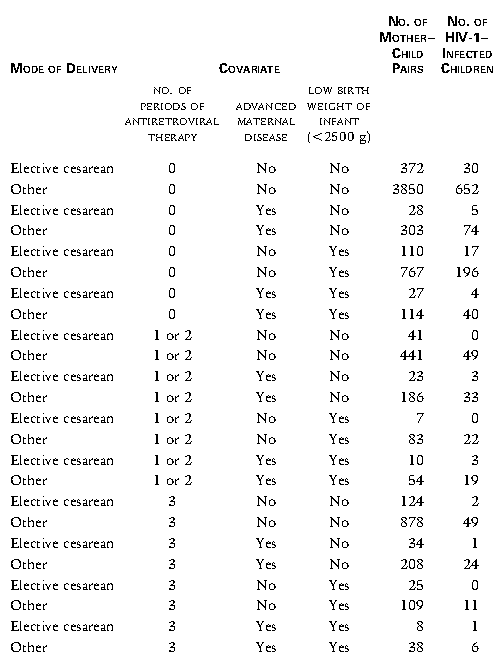
\includegraphics[scale=1.1]{hivtable.pdf}
\end{figure}




\begin{table}[H]
	\centering
	\begin{tabular}{lcc|c}
			     & Exposed  &   Unexposed & Total  \\		
		Cases    & $a_i$ &  $b_i$ & $M_{1i}$ \\
		Controls & $c_i$ 	& $d_i$  	& $M_{0i}$ 	\\	
		\hline
		Total & $N_{1i}$ & $N_{0i}$ 	& $T_i$
	\end{tabular}
\end{table}


$OR_{MH} = \frac{\sum_i \frac{a_i d_i}{T_i}}{\sum_i \frac{b_i c_i}{T_i}}$ \\ \ \\
$RR_{MH} = \frac{\sum_i \frac{a_i N_{0i}}{T_i}}{\sum_i \frac{b_i N_{1i}}{T_i}}$


\begin{enumerate}\compresslist
	\item You only have access to a hand calculator. You are asked to provide a evidence on whether Elective cesarean is protective for HIV vertical transmission or not. Explain what you would do. 
	\item Several regression outputs are shown below. For each, provide the regression equation in terms of the population parameters being fit. 
	\item When applicable, explain what the \texttt{Estimate} for \texttt{caesarian} represents. 
	\item What statement can you make about c-sections and HIV vertical transmission based on these models? Provide statistical evidence to support your answer.  
\end{enumerate}

\clearpage

\begin{knitrout}\small
\definecolor{shadecolor}{rgb}{0.969, 0.969, 0.969}\color{fgcolor}
\begin{verbatim}
## Call:
## glm(formula = cbind(n.hivpos, n.hivneg) ~ 1, family = binomial(link = logit), 
##     data = ds)
## 
## Coefficients:
##             Estimate Std. Error z value Pr(>|z|)    
## (Intercept)   -1.671      0.031     -54   <2e-16 ***
## ---
## Signif. codes:  0 '***' 0.001 '**' 0.01 '*' 0.05 '.' 0.1 ' ' 1
## 
## (Dispersion parameter for binomial family taken to be 1)
## 
##     Null deviance: 293.95  on 23  degrees of freedom
## Residual deviance: 293.95  on 23  degrees of freedom
## AIC: 387.8
## 
## Number of Fisher Scoring iterations: 4
\end{verbatim}

\end{knitrout}


\begin{knitrout}\small
\definecolor{shadecolor}{rgb}{0.969, 0.969, 0.969}\color{fgcolor}
\begin{verbatim}
## Call:
## glm(formula = cbind(n.hivpos, n.hivneg) ~ caesarian, family = binomial(link = logit), 
##     data = ds)
## 
## Coefficients:
##             Estimate Std. Error z value Pr(>|z|)    
## (Intercept)   -1.606      0.032   -50.2   <2e-16 ***
## caesarian     -0.815      0.132    -6.2    7e-10 ***
## ---
## Signif. codes:  0 '***' 0.001 '**' 0.01 '*' 0.05 '.' 0.1 ' ' 1
## 
## (Dispersion parameter for binomial family taken to be 1)
## 
##     Null deviance: 293.95  on 23  degrees of freedom
## Residual deviance: 247.78  on 22  degrees of freedom
## AIC: 343.7
## 
## Number of Fisher Scoring iterations: 4
\end{verbatim}

\end{knitrout}




\clearpage

\vspace{-0.3in}

\begin{knitrout}\small
\definecolor{shadecolor}{rgb}{0.969, 0.969, 0.969}\color{fgcolor}
\begin{verbatim}
## Call:
## glm(formula = cbind(n.hivpos, ds$n.hivneg) ~ caesarian + ART1or2 + 
##     ART3 + m.advancedHIV + c.LBW, family = binomial(link = logit), 
##     data = ds)
## 
## Coefficients:
##               Estimate Std. Error z value Pr(>|z|)    
## (Intercept)     -1.608      0.041   -39.6   <2e-16 ***
## caesarian       -0.852      0.134    -6.3    2e-10 ***
## ART1or2         -0.362      0.106    -3.4    6e-04 ***
## ART3            -1.178      0.114   -10.3   <2e-16 ***
## m.advancedHIV    0.535      0.090     6.0    3e-09 ***
## c.LBW            0.581      0.075     7.8    9e-15 ***
## ---
## Signif. codes:  0 '***' 0.001 '**' 0.01 '*' 0.05 '.' 0.1 ' ' 1
## 
## (Dispersion parameter for binomial family taken to be 1)
## 
##     Null deviance: 293.945  on 23  degrees of freedom
## Residual deviance:  18.393  on 18  degrees of freedom
## AIC: 122.3
## 
## Number of Fisher Scoring iterations: 4
\end{verbatim}

\end{knitrout}

\vspace{-0.22in}

\begin{knitrout}\small
\definecolor{shadecolor}{rgb}{0.969, 0.969, 0.969}\color{fgcolor}
\begin{verbatim}
## Call:
## glm(formula = cbind(n.hivpos, ds$n.hivneg) ~ caesarian + ART1or2 + 
##     ART3 + m.advancedHIV + c.LBW, family = binomial(link = log), 
##     data = ds)
## 
## Coefficients:
##               Estimate Std. Error z value Pr(>|z|)    
## (Intercept)     -1.793      0.034   -53.2   <2e-16 ***
## caesarian       -0.720      0.119    -6.0    2e-09 ***
## ART1or2         -0.278      0.087    -3.2    0.001 ** 
## ART3            -1.016      0.104    -9.8   <2e-16 ***
## m.advancedHIV    0.409      0.068     6.0    2e-09 ***
## c.LBW            0.453      0.057     7.9    2e-15 ***
## ---
## Signif. codes:  0 '***' 0.001 '**' 0.01 '*' 0.05 '.' 0.1 ' ' 1
## 
## (Dispersion parameter for binomial family taken to be 1)
## 
##     Null deviance: 293.945  on 23  degrees of freedom
## Residual deviance:  21.295  on 18  degrees of freedom
## AIC: 125.2
## 
## Number of Fisher Scoring iterations: 5
\end{verbatim}

\end{knitrout}


\clearpage

\section{Smoking among women in Whickham, UK}
Consider the following \textit{age stratified} mortality data (Rothman, Table 1-2) from a study that looked at smoking habits of residents of Whickham, England, in the period 1972-1974 and then tracked the survival over the next 20 years of those who were interviewed. 


\begin{table}[h]
	\centering
	\begin{tabular}{lcccc}
		 &  &   \multicolumn{2}{c}{Smoking} &  \\		
		Age & Vital Status &  Yes & No & Total \\
		18-24 	& Dead 	& 2  	& 1 	& 3 	\\	
		 		& Alive & 53  	& 61 	& 114 	\\
		 		& Risk & 0.04  	& 0.02 	& 0.03 	\\
		 		\hline
		25-34 	& Dead 	& 3  	& 5 	& 8 	\\	
& Alive & 121  	& 152 	& 273 	\\
& Risk & 0.02  	& 0.03 	& 0.03 \\
\hline 			
35-44 	& Dead 	& 14  	& 7 	& 21 	\\	
& Alive & 95  	& 114 	& 209 	\\
& Risk & 0.13  	& 0.06 	& 0.09 \\
\hline
45-54 	& Dead 	& 27  	& 12 	& 39 	\\	
& Alive & 103  	& 66 	& 169 	\\
& Risk & 0.21  	& 0.15 	& 0.19 \\
		 		\hline
55-64 	& Dead 	& 51  	& 40 	& 91 	\\	
& Alive & 64  	& 81 	& 145 	\\
& Risk & 0.44  	& 0.33 	& 0.39 \\
		 		\hline
65-74 	& Dead 	& 29  	& 101 	& 130 	\\	
& Alive & 7  	& 28 	& 35 	\\
& Risk & 0.81  	& 0.78 	& 0.79 \\
		 		\hline
75+ 	& Dead 	& 13  	& 64 	& 77 	\\	
& Alive & 0  	& 0 	& 0 	\\
& Risk & 1.00  	& 1.00 	& 1.00 \\
\hline
	\end{tabular}
\end{table}



\begin{enumerate}\compresslist
	\item Calculate the crude odds ratio for smoking vs. not smoking. 
	\item You are asked to provide evidence on whether smoking affects mortality. Provide a full analysis plan, including a regression model with population parameters, the parameter of interest, what the data should look like to fit in a regression routine and the \texttt{R} code for the regression routine. State concretely what you would provide as evidence. 
\end{enumerate}






\end{document}
